%****************************************************************%
% FILE: modelli_previsione.tex                                   %
%****************************************************************%
\documentclass[./main.tex]{subfiles}

\begin{document}

% ISSOS ??? nah, tanto non l'hanno ancora messo

I modelli di previsione permettono di predire il tempo climatico futuro. L'applicazione visualizzerà i diagrammi di due sistemi: \textbf{Nettuno} per il mar Mediterraneo, \textbf{Henetus} per il nord del mar Adriatico. Quando si pensa alle previsioni la prima cosa che viene in mente è se ci sarà il sole o la pioggia. Invece, le due strutture si occupano prevalentemente di onde, Nettuno anche del vento. Rivelazione un po' deludente, ma anche loro sono importanti! Ad esempio Henetus viene utilizzato per predire l'acqua alta a Venezia, fortemente influenzata dal moto ondoso del litorale veneto\footcite[2972-2976]{henetus-wave}. Nei paragrafi successivi saranno analizzati entrambi in modo approfondito.

\paragraph{Nettuno.}

Nettuno è un sistema di previsione dei venti e delle onde per il mar Mediterraneo. Esso è operativo dal 2009 e, ogni 24 ore, produce le previsioni fino a 72 ore delle condizioni meteo. Il modello meteorologico \textbf{COSMO} (\textit{Consortium for small-Scale MOdelling}) si occupa di rilevare le condizioni del vento, mentre il modello spettrale di terza generazione \textbf{WAM} (\textit{Mediterranean Wave Forecast}) valuta i campi d'onda\footcite[\url{https://www.ismar.cnr.it/infrastrutture/modellistica/modelli-operativi/\#2}]{website-ismar-cnr}.\par

Il mar Mediterraneo si estende per più di 3500 km in longitudine (6°W–36.5°E) e più di 1600 km in latitudine (30°–46°N). Nettuno garantisce la copertura dell'intera area geografica del Mediterraneo. Nettuno viene integrato due volte al giorno (a partire dalle 00:00 e dalle 12:00 UTC) per una previsione di 72 ore\footcite[3130-3132]{nettuno-analysis}.\par

I dati non sono pubblici. ISMAR-CNR ha fornito, per conto dell'ente privato che gestisce i dati, alcuni file di esempio riguardanti le misurazioni effettuate in un arco temporale di 10 giorni nel mese di aprile 2024. Ovviamente il problema della mancanza di dati persiste. Non è possibile far funzionare un'applicazione che necessita di dati in continuo aggiornamento (in questo caso anche di previsione!) avendo a disposizione solo alcuni dati vecchi; l'unica nota positiva è la possibilità di analizzare i file per essere preparati quando si avrà a disposizione una sorgente reale da cui reperirli. I dati seguono il formato \textit{GRIB}. \textbf{GRIB} (\textit{General Regularly distributed Information in Binary form}) appartiene ai formati standard per l'archiviazione e lo scambio di dati meteorologici su griglia. Un GRIB file è definito dalla concatenazione di più file con estensione \textit{.grib} o \textit{.grb}\footcite[\url{https://confluence.ecmwf.int/display/CKB/What+are+GRIB+files+and+how+can+I+read+them}]{website-ecmwf-confluence}. Il nome di ogni file segue il formato compresso \textit{grib\_WAM\_yyyymmddhh.tar.bz2}. Esso sta ad indicare che il contenuto del file si riferisce alle previsioni del modello di onde WAM, e contiene dati in formato grib. La data (\textit{yyyymmdd}) fa riferimento al giorno in cui è stata fatta la previsione. Di seguito un numero (\textit{hh}) indica l'orario, il quale può essere mezzanotte (ore 00) oppure mezzogiorno (ore 12). In \autoref{fig:thunar_GRIB_nettuno_compressed} è presente la lista dei file ricevuti. L'elemento selezionato ha nome \textit{grib\_WAM\_2024041412.tar.bz2} e sta ad indicare il file con la previsione del giorno 14 aprile 2024 alle ore 12. All'interno del file sono contenuti esattamente 25 file grib del tipo \textit{WAMyyyymmdd0000\_hhh.grb}, ognuno dei quali si riferisce all'ora della previsione (\textit{hhh}) con passo temporale di 3 ore, da 000 a 072. Questi sono i dati reali dei campi d'onda e di vento nel Mediterraneo. 
\begin{figure}[!ht]
\noindent \begin{minipage}{\textwidth}
\vspace{1cm}
\centering
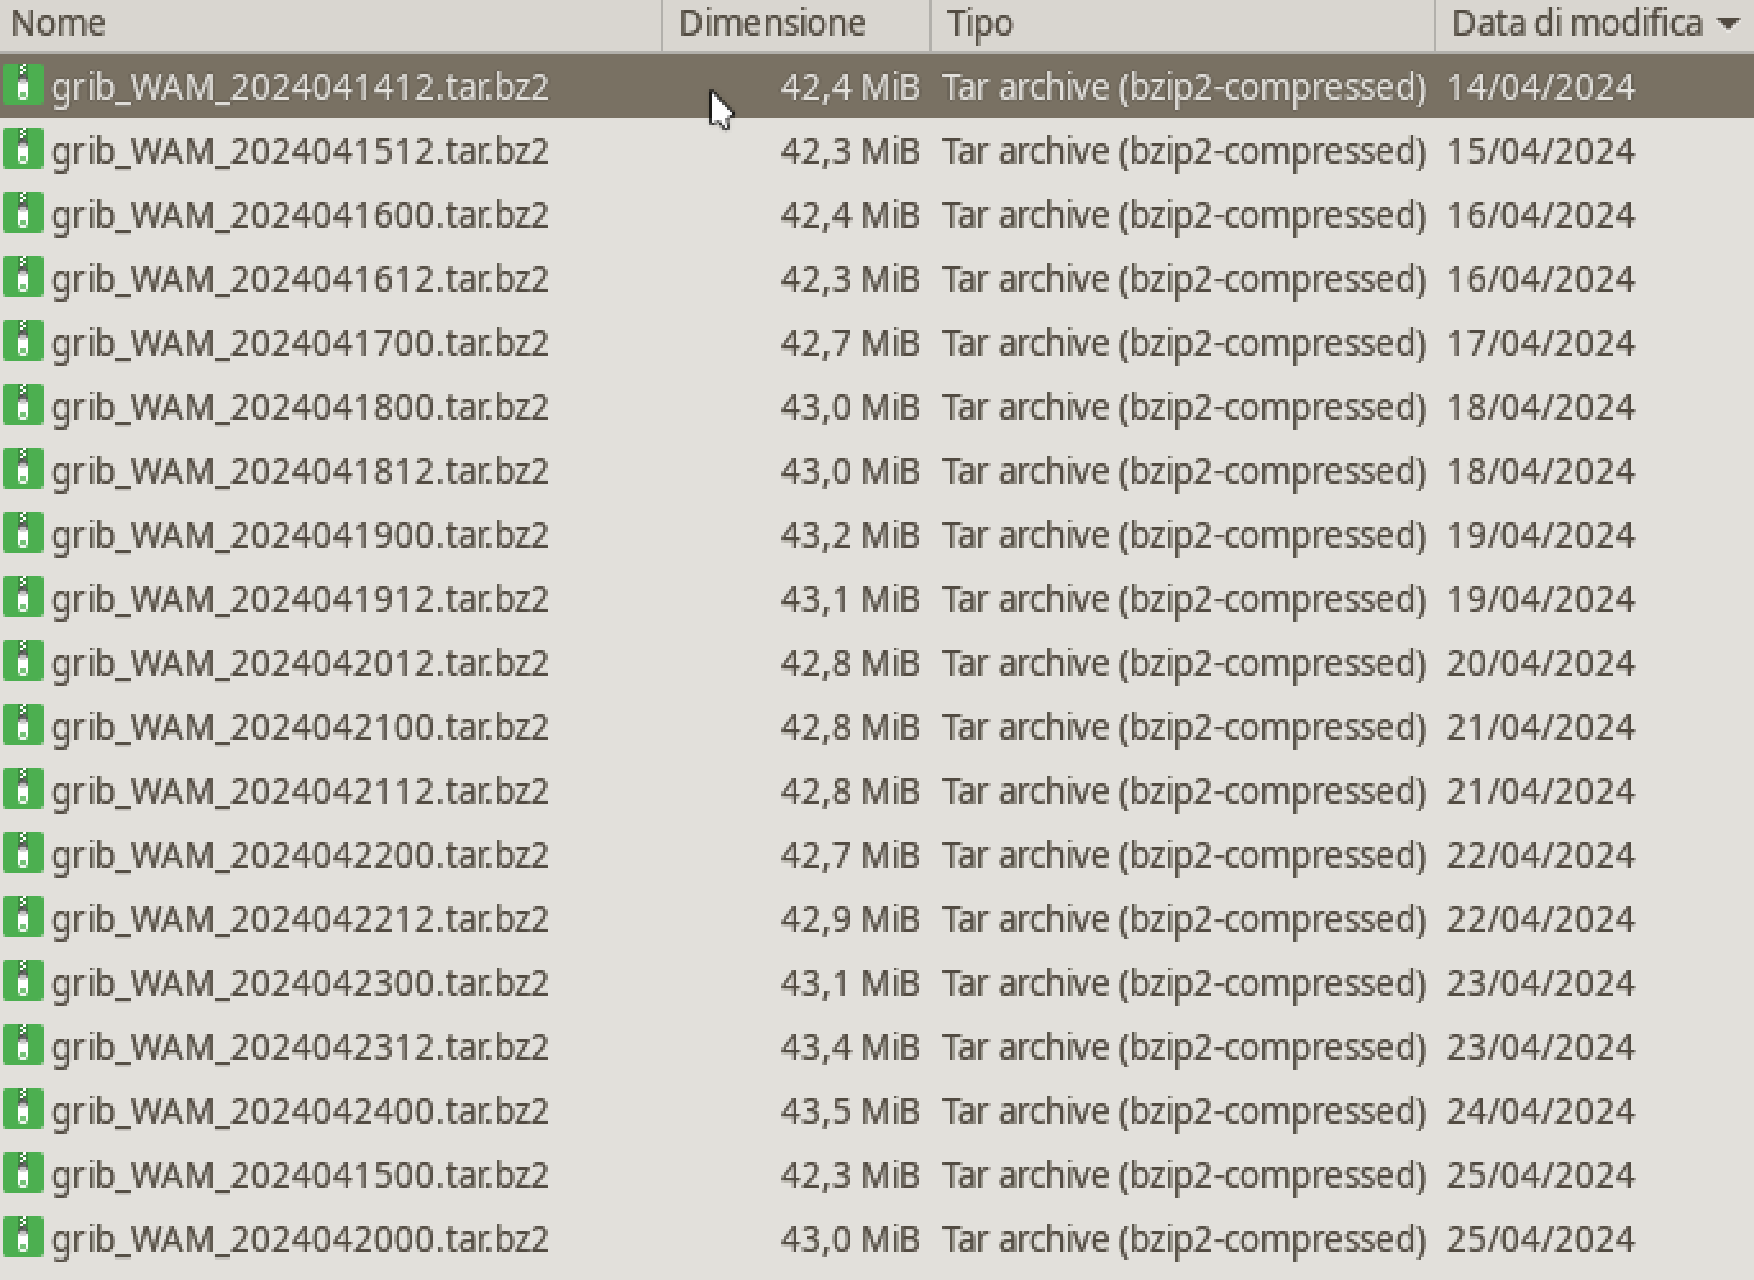
\includegraphics[width=0.8\textwidth]{images/thunar_GRIB_nettuno_compressed.pdf}
\captionsetup{font=small, hypcap=false}
\captionof{figure}{File compressi contenenti le previsioni di Nettuno con dati in formato grib dal 14 aprile al 24 aprile 2024\protect\footnote{Fonte: screenshot dell'autrice.}.}
\label{fig:thunar_GRIB_nettuno_compressed}
\end{minipage}
\vspace{0.25cm}
\end{figure}

In \autoref{fig:thunar_GRIB_nettuno_14042024} si possono osservare i 25 file relativi al 14 aprile 2024 alle ore 12. Ogni file grib contiene un certo numero di parametri, identificati da un numero, ad indicare le misurazioni effettuate:
\begin{itemize}
    \item \textbf{140229}: altezza significativa, in metri, delle onde combinate del vento e del moto ondoso (\textit{swh -- Significant height of combined wind waves and swell});
    \item \textbf{140230}: direzione media dell'onda (mwd -- \textit{Mean wave direction});
    \item \textbf{140232}: periodo medio, in secondi, dell'onda (\textit{mwp -- Mean wave period}). Indica il tempo medio impiegato da due creste d'onda consecutive, sulla superficie dell'oceano/mare, per attraversare un punto fisso;
    \item \textbf{140249}: direzione del vento (\textit{dwi -- 10 metre wind direction}). Rappresenta la direzione da cui soffia il vento, in gradi in senso orario dal nord geografico, ad un'altezza di dieci metri sopra la superficie della Terra;
    \item \textbf{140231}: periodo, in secondi, di picco dell'onda (\textit{pp1d --Peak wave period}). Questo parametro rappresenta il periodo delle onde oceaniche più energetiche generate dai venti locali;
    \item \textbf{140233}: coefficiente di drag con le onde (\textit{cdww -- Coefficient of drag with waves}). Indica la resistenza che le onde dell'oceano esercitano sull'atmosfera.  A volte viene anche chiamato "coefficiente di attrito". Non ha un'unità di misura;
    \item \textbf{140245}: velocità del vento (\textit{wind -- 10 metre wind speed}). Questo parametro è la velocità orizzontale del vento in metri al secondo ($m*s^{-1}$), ad un'altezza di dieci metri sopra la superficie della Terra;
    \item \textbf{131}: componente U del vento (\textit{u -- U component of wind}). È la velocità orizzontale dell'aria che si muove verso est, espressa in metri al secondo ($m*s^{-1}$).  Un segno negativo indica quindi un movimento d'aria verso ovest;
    \item \textbf{132}: componente V del vento (\textit{v -- V component of wind}). È la velocità orizzontale dell'aria che si muove verso nord, espressa in metri al secondo ($m*s^{-1}$).  Un segno negativo indica quindi un movimento d'aria verso sud.
\end{itemize}

I parametri sono divisi in tabelle in base al settore nel quale sono raccolti i dati. Le prime tre cifre del numero del parametro indicano la tabella di appartenenza, ad eccezione della tabella standard che non ha un numero identificativo.  In questo caso i prime sette parametri appartengono alla tabella numero 140 relativa alle onde, gli ultimi due (componenti U e V) alla tabella standard. L'elenco completo dei possibili parametri e tabelle si può trovare nel database gestito dal Centro europeo per le previsioni meteorologiche a medio termine\footcite[\url{https://codes.ecmwf.int/grib/param-db/?encoding=grib1}]{website-ecmwf-grib} (ECMWF) -- European Centre for Medium-range Weather Forecasts. \par


\begin{figure}[!ht]
\noindent \begin{minipage}{\textwidth}
\vspace{1cm}
\centering
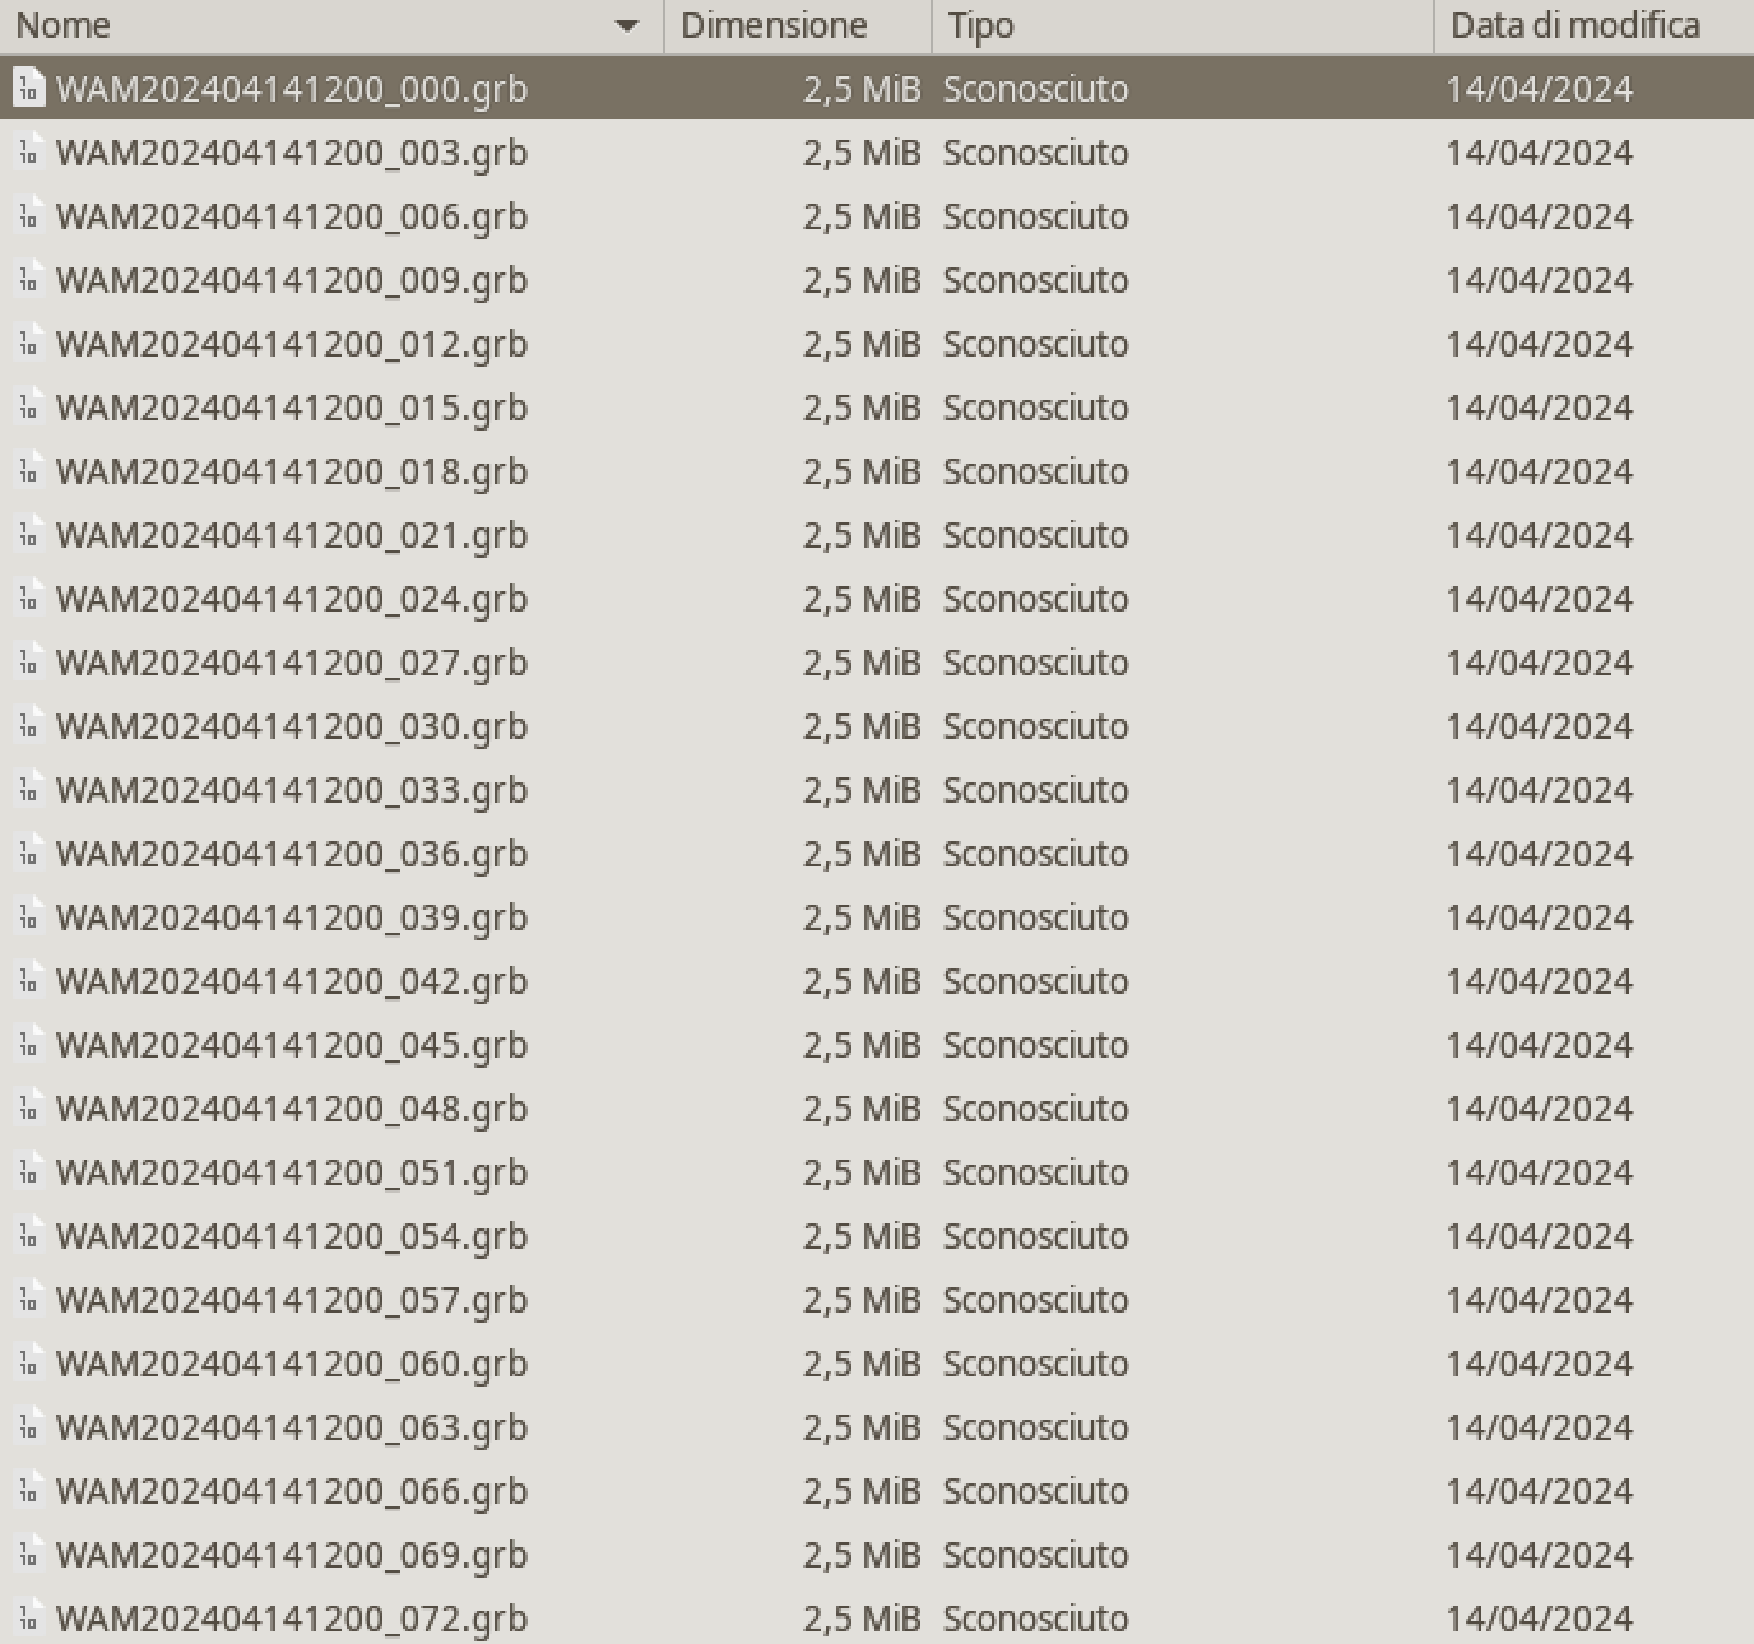
\includegraphics[width=0.8\textwidth]{images/thunar_GRIB_nettuno_14042024.pdf}
\captionsetup{font=small, hypcap=false}
\captionof{figure}{Contenuto del file grib\_WAM\_2024041412.tar.bz2: 25 file grib di dati misurati con passo temporale di 3 ore, da 000 a 072.\protect\footnote{Fonte: screenshot dell'autrice.}.}
\label{fig:thunar_GRIB_nettuno_14042024}
\end{minipage}
\vspace{0.25cm}
\end{figure}

In realtà, per \textit{Ismar Data} non tutti i parametri sono rilevanti. L'applicazione dovrà visualizzare un solo grafico dinamico (posto su una cartina geografica) relativo all'altezza delle onde e all'intensità del vento, in particolare l'altezza delle onde sarà rappresentata da un livello colorato e l'intensità del vento dalle freccette ad indicarne la direzione (verso della freccia) e intensità (lunghezza della freccia). Questi dati si ottengono usando i parametri \textbf{140229} e \textbf{140230} per le onde, mentre \textbf{131} e \textbf{132} per il vento. In \autoref{fig:plot_pygrib_nettuno_202404141200} è presente un esempio dei risultati che si ottengono utilizzando i dati a disposizione.\par

\begin{figure}[!ht]
\noindent \begin{minipage}{\textwidth}
\vspace{1cm}
\centering
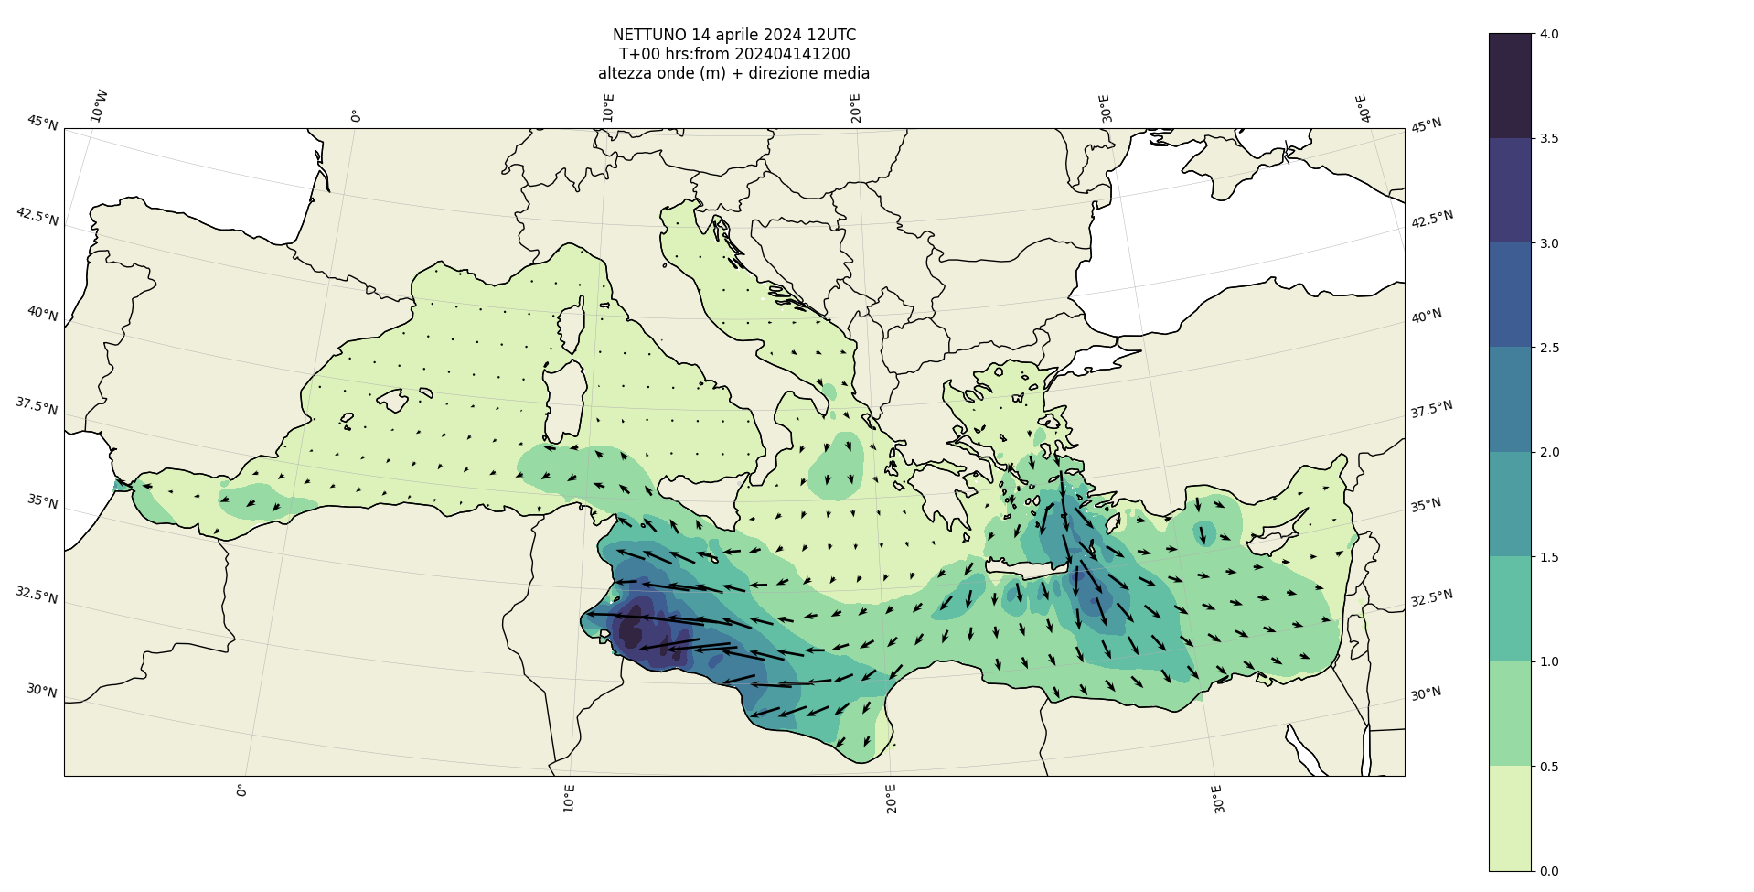
\includegraphics[width=\textwidth]{images/plot_pygrib_nettuno_202404141200.pdf}
\captionsetup{font=small, hypcap=false}
\captionof{figure}{Esempio di grafico relativo all'altezza delle onde e all'intensità del vento misurate da Nettuno il 14 aprile 2024.\protect\footnote{Fonte: screenshot dell'autrice.}.}
\label{fig:plot_pygrib_nettuno_202404141200}
\end{minipage}
\vspace{0.25cm}
\end{figure}

\paragraph{Henetus - Mar Adriatico.}
\textbf{Henetus}, dal 1996, è il sistema di previsione del moto ondoso nel Mar Adriatico. Si basa sui campi di vento in formato \textit{\textbf{ECMWF}} (\textit{European Centre for Medium-range Weather Forecasts}) ed è in grado di ottenere risultati fino a cinque giorni di previsione\footcite[\url{https://www.ismar.cnr.it/infrastrutture/modellistica/modelli-operativi/\#3}]{website-ismar-cnr}.\par

Il mar Adriatico si estende per circa 740km di lunghezza e 200km di larghezza (vedi area in \autoref{fig:adriatico_grid}). Le previsioni utilizzate dal CNR sono quelle riguardanti il quadrante nord, osservato dalla torre oceanografica di ISMAR\footcite[2967]{henetus-wave}.\par

\begin{figure}[!ht]
\noindent \begin{minipage}{0.5\textwidth}
\vspace{1cm}
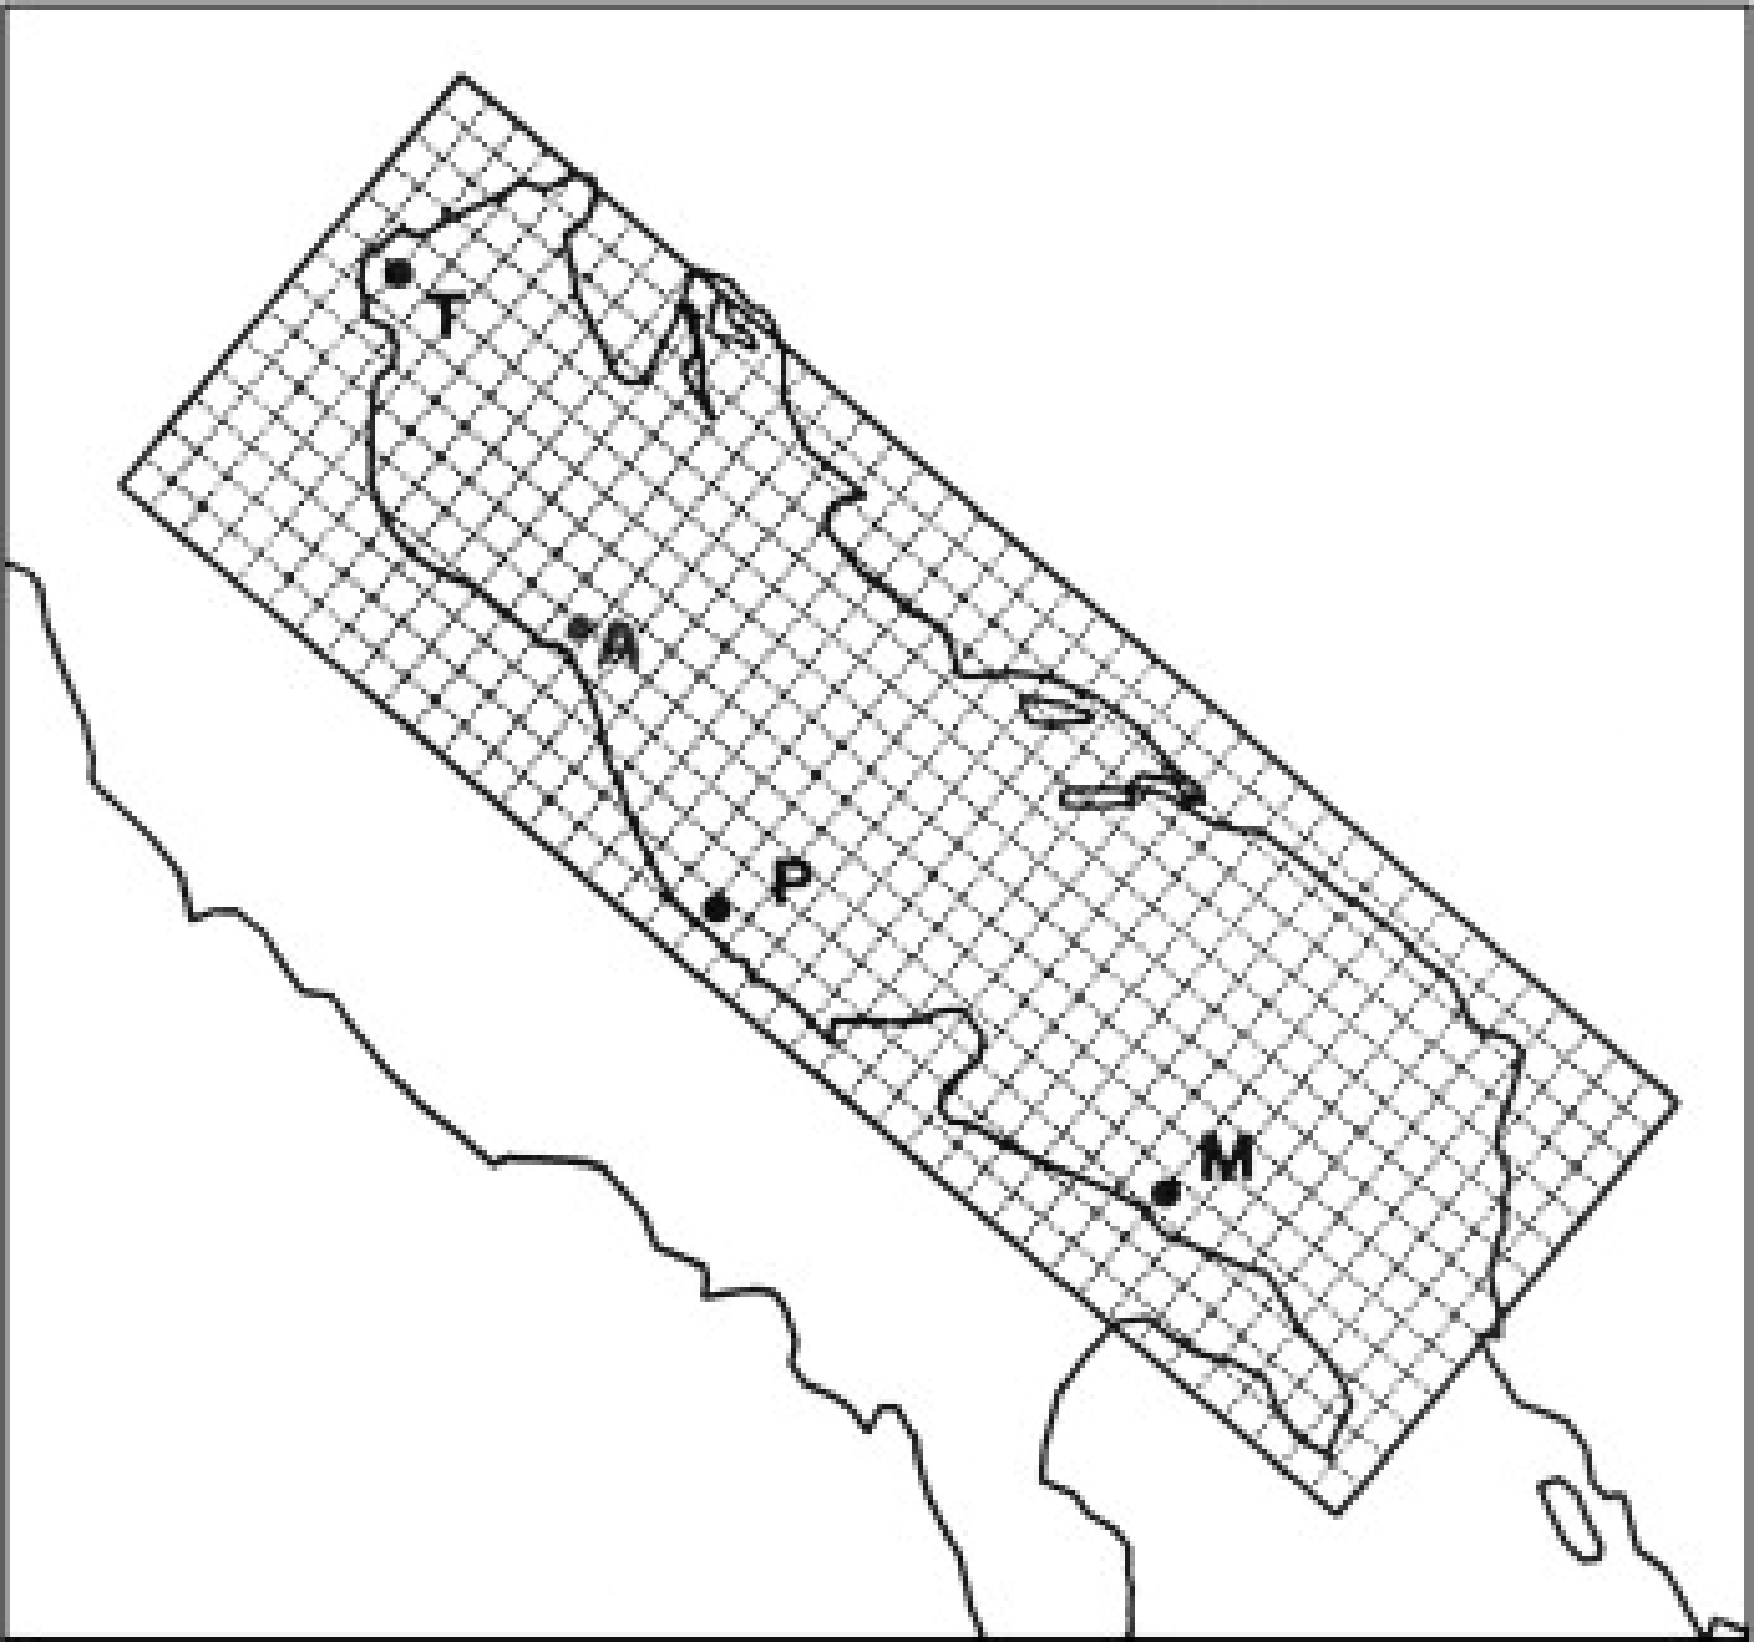
\includegraphics[width=\textwidth]{images/mar_adriatico_grid.pdf}
\captionsetup{font=small, hypcap=false}
\captionof{figure}{Geometria del mar Adriatico.}
\label{fig:adriatico_grid}
\end{minipage}
\hspace{0.05\textwidth}
\begin{minipage}{0.4\textwidth}
\begin{small}
Immagine rappresentante il quadrante del mar Adriatico. I puntini rappresentano la posizione della torre oceanografica di ISMAR (T) e delle boe poste ad Ancona (A), Pescara (P) e Monopoli (M).
\end{small}
\end{minipage}
\vspace{0.25cm}
\end{figure}

I dati non sono pubblici. Anche in questo caso il cliente ha fornito, per conto dell'ente privato che gestisce i dati, alcuni file di esempio riguardanti le misurazioni effettuate in un arco temporale di quattro mesi, dal 14 gennaio al 23 aprile 2024. Questo, ovviamente, comporta le stesse problematiche presenti per i file di Nettuno. Ogni file contiene i campi d'onda relativi a 24 ore sull'area del Mar Adriatico. Il nome di ogni file segue il formato \textit{OPEyymmdd12xxxx.gz} dove OPE significa run/previsione OPERATIVA e \textit{gz} indica la compressione del file. La data (\textit{yymmdd}) si riferisce all'anno, mese e giorno dell'\textit{ultimo} campo della previsione. Il numero, sempre \textit{12}, indica l'ora di \textit{inizio} della previsione.  Ne risulta che il giorno di inizio è in realtà il precedente alla data presente nel nome del file, in quanto quest'ultima indica appunto la data dell'\textit{ultimo} campo della previsione (al termine delle 24 ore di monitoraggio). Infine i quattro numeri \textit{(xxxx}) possono assumere sei diversi valori di diverso significato:
\begin{itemize}
    \item 0000: \textit{analisi} in ore;
    \item 0024: \textit{previsione} in ore del giorno 1;
    \item 0048: \textit{previsione} in ore del giorno 2;
    \item 0072: \textit{previsione} in ore del giorno 3;
    \item 0096: \textit{previsione} in ore del giorno 4;
    \item 0120: \textit{previsione} in ore del giorno 5.
\end{itemize}

In \autoref{fig:thunar_OPE_henetus_compressed} è presente l'elenco dei file ricevuti. Il file selezionato, \textit{OPE240114120072.gz}, rappresenta la previsione del terzo giorno (\textit{0072}) a partire dal giorno 13/01/2024 alle ore 12; quindi la previsione del giorno 16/01/2024.

\begin{figure}[!ht]
\noindent \begin{minipage}{\textwidth}
\vspace{1cm}
\centering
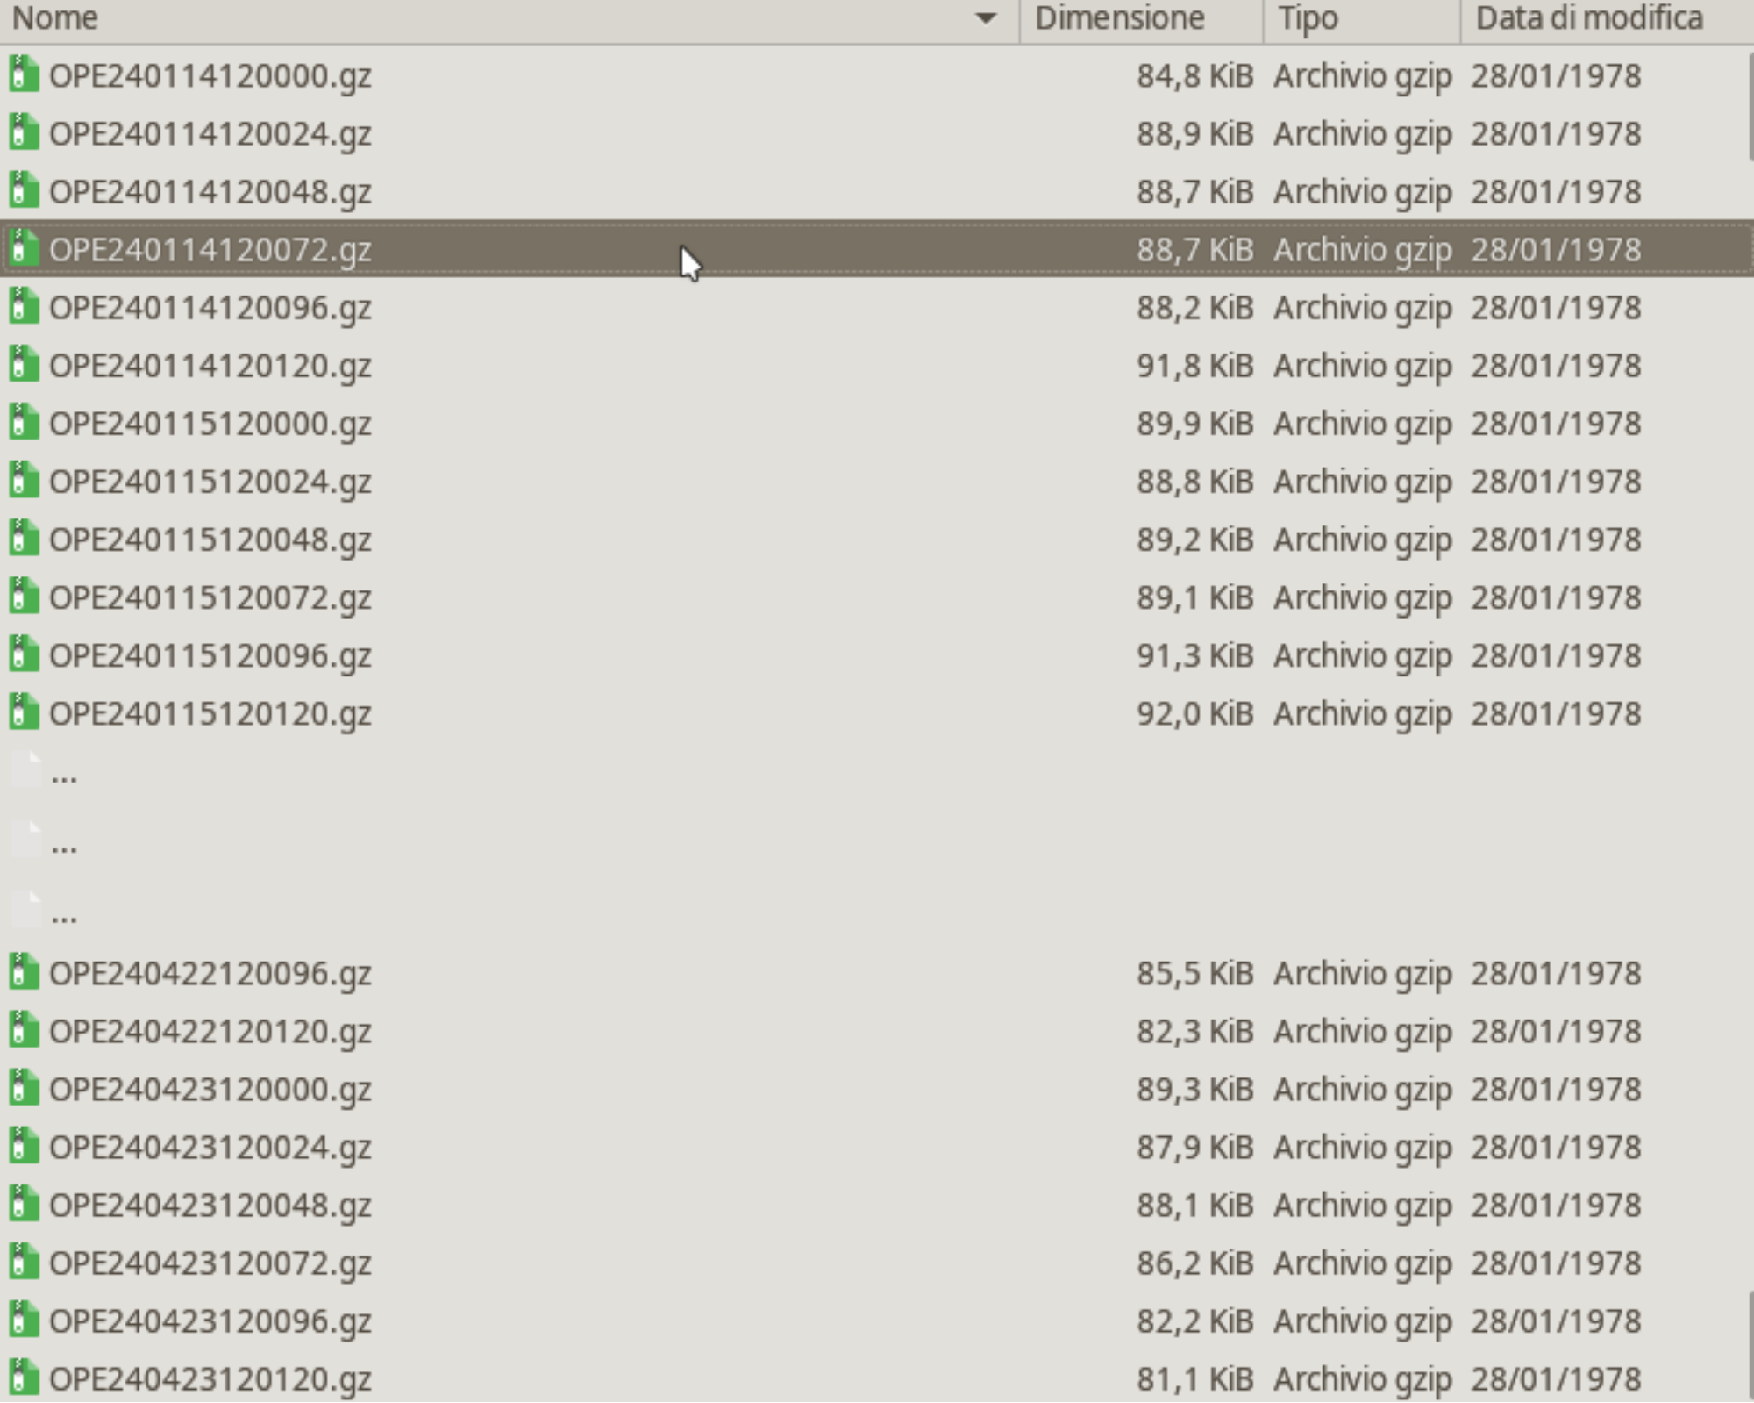
\includegraphics[width=0.8\textwidth]{images/thunar_OPE_henetus_compressed.pdf}
\captionsetup{font=small, hypcap=false}
\captionof{figure}{File compressi contenenti i campi d'onda rilevati dal sistema Henetus dal 14 gennaio al 23 aprile 2024.\protect\footnote{Fonte: screenshot dell'autrice.}.}
\label{fig:thunar_OPE_henetus_compressed}
\end{minipage}
\vspace{0.25cm}
\end{figure}

All'interno di questi file compressi è presente un unico file contenente le reali misurazioni. Il nome corrisponde al relativo file \textit{OPEyymmdd12xxxx.gz}, a meno dell'estensione. Il contenuto di questi file, a prima vista, risulta essere particolarmente complicato. Il gestore di questi dati ha quindi fornito una breve guida per aiutare gli sviluppatori nella comprensione. Un esempio, relativo al file \textit{OPE240114120072} contenuto nel file selezionato in \autoref{fig:thunar_OPE_henetus_compressed}, è mostrato in \autoref{fig:OPE_henetus_example_2401161500}. I campi d'onda sono raggruppati a intervalli di 3 ore e, per ogni ora, sono presenti quattro matrici di dimensione 97x73. Vengono considerati quattro parametri d'onda:
\begin{itemize}
    \item \textbf{ONDAHS}: altezza onda;
    \item \textbf{ONDADIR}: direzione onda;
    \item \textbf{ONDAFM}: frequenza media dell'onda;
    \item \textbf{ONDAFP}: frequenza di picco dell'onda.
\end{itemize}
Ogni matrice contiene un parametro d'onda. I limiti geografici sono rappresentati da:
\begin{itemize}
    \item latitudine: 40.0 - 46.00  gradi Nord;
    \item longitudine:  12.00 - 20.00  gradi Est.
\end{itemize}
con passo geografico 0.083 x 0.083  (1/12 x 1/12 di gradi) e il punto (1,1), posto in basso a sinistra, indica il punto sud-ovest.

\begin{figure}[!ht]
\noindent \begin{minipage}{\textwidth}
\vspace{1cm}
\centering
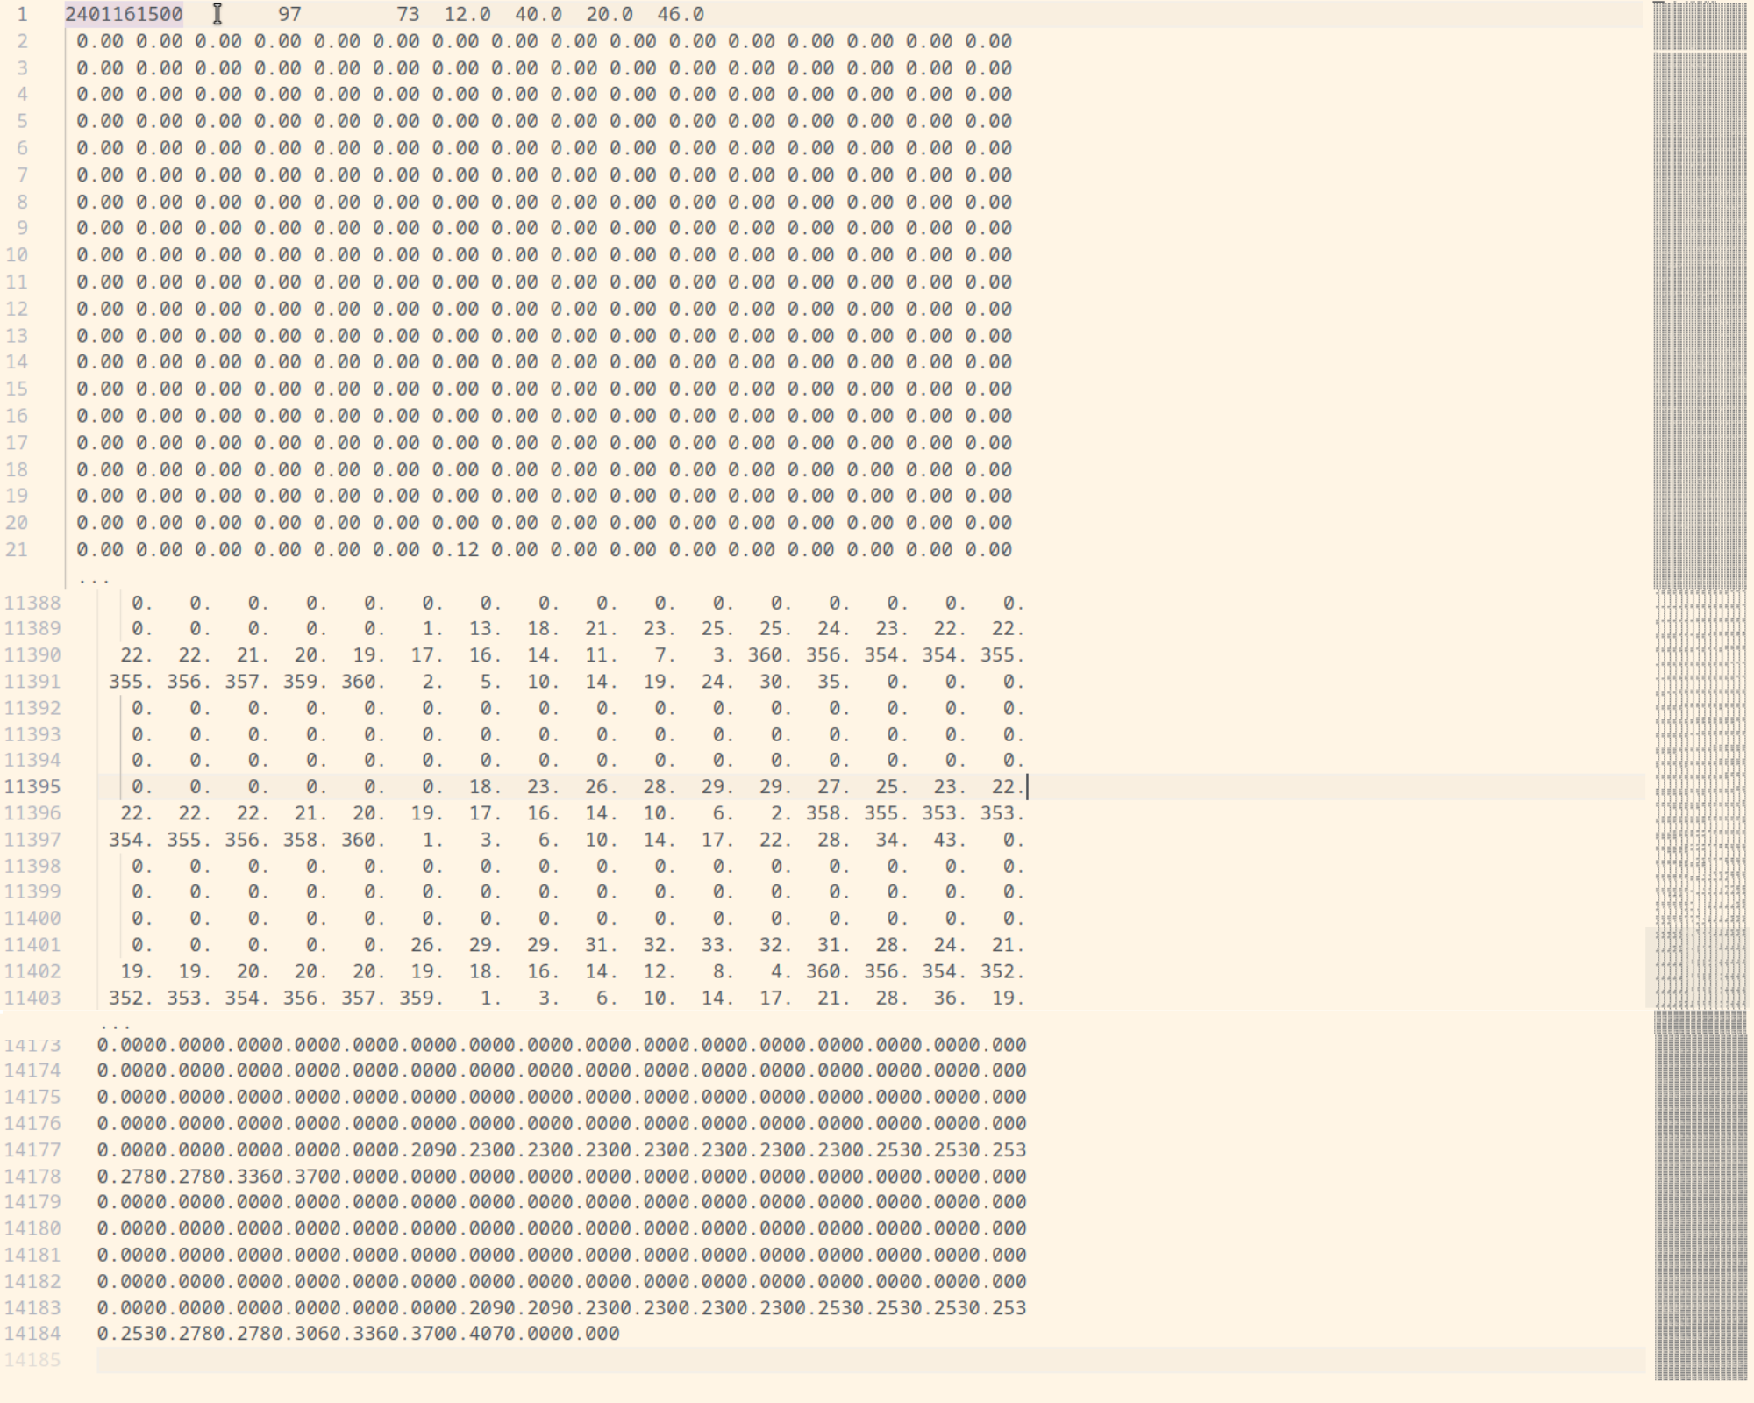
\includegraphics[width=0.8\textwidth]{images/OPE_henetus_example_2401161500.pdf}
\captionsetup{font=small, hypcap=false}
\captionof{figure}{Esempio delle misurazioni dei campi d'onda di Henetus rappresentanti la previsione del 16/01/2024; terzo giorno (0072) a partire dal giorno 13/01/2024 alle ore 12. \protect\footnote{Fonte: screenshot dell'autrice.}.}
\label{fig:OPE_henetus_example_2401161500}
\end{minipage}
\vspace{0.25cm}
\end{figure}

La prima riga di ogni file contiene data e ora, dimensioni della matrice e limiti geografici. Da notare che la data non è la stessa del nome del file. Infatti si riferisce esattamente al giorno della previsione. Nell'esempio in questione si ha \textit{2401161500        97        73  12.0  40.0  20.0  46.0}. In questo caso la data è 16/01/2024 alle ore 15:00. Che indica esattamente la data e il giorno della previsione la previsione del terzo giorno (\textit{0072}) a partire dal giorno 13/01/2024 alle ore 12 (nome del file \textit{OPE240114120072}). Le righe successive contengono le matrici, con i parametri d'onda, e sono lette riga per riga dall'alto verso il basso (ovvero da nord a sud e da ovest ad est). Il grafico richiesto dal cliente è relativo all'altezza delle onde, quindi le uniche matrici rilevanti sono ONDAHS e ONDADIR.\par

\end{document}